
\chapter{Determinants}

\section{The Determinant Function}

We are all familiar with functions lilke $f(x) = \sin x$ and $f(x)=x^2$,
which associate a real number $f(x)$ with a real value of the variable
$x$.  Since both $x$ and $f(x)$ assume only real values, such functions
can be described as real-valued functions of a matrix variable, that is,
functions that associate a real number $f(X)$ with a matrix $X$.

Before we shall be able to define the determinant function, it will be
necessary to establish some results concerning permutations.

\begin{definition}
A {\it permutation} of the set of integers $\{1,2,\ldots,n\}$ is an
arrangement of these integers in some order without ommissions or
repetitions.
\end{definition}

\begin{example}
There are six different permutations of the set of integers $\{1,2,3\}$.
These are
%
\begin{alignat}{2}
 (1,2,3) & (2,1,3) & (3,1,2) \\
 (1,3,2) & (2,3,1) & (3,2,1)
\end{alignat}
\end{example}

One convenient method of systematically listing permutations is to use a
{\it permutation tree}.  This method will be illustrated in our next
example.

\begin{example}
List all permutations of the set of integers $\{1,2,3,4\}$

%
% --------------------------------------------------------------
% Note that if we have more than an single instance of something
% like the solution below, we could create a theorem definition
% using the commands:
%
%   \theoremstyle{remark}              % italic headings
%   \newtheorem*{solution}{Solution}   % heading is unnumbered
%
% --------------------------------------------------------------
%

\noindent{\it Solution.}\quad
By drawing a permutation tree with each branch representing all four
numbers, we see that there are a total of 24 possible permutations.
\end{example}


\section{Evaluating Determinants by Row Reduction}

In this section we show that the determinant of a matrix can be
evaluated by reducing the matrix to row-echelon form.  This method is of
importance since it avoids the lengthy computations involved directly
applying the determinant definition.

We first consider two class of matrices whose determinants can be easily
evaluated, regardless of the size of the matrix.

\begin{theorem}
If $A$ is any square matrix that contains a row of zeros, then
$\det(A)=0$.
\end{theorem}

\begin{theorem}
If $A$ is an $n\times n$ triangular matrix, then $\det(A)$ is the
product of the entries on the main diagonal; that is $\det(A)=
a_{11}a_{22} \cdots a_{mn}$.
\end{theorem}

\begin{example}
Evaluate $\det(A)$ where
\begin{equation}
  A =  \left[ \  \begin{matrix} 1 & 2 \\ 3 & 4 \end{matrix}
		\ \right]
\end{equation}
\end{example}


\subsection{Some Final Conclusions}

It should be evident from the examples in this section that whenever a
square matrix has two proportional rows (like the first and second rows
of $A$), it is possible to introduce a row of zeros by adding a suitable
mutliple of one of these rows to the other.  Thus, if a square matrix
has two proportional rows, its determinant is zero.

In the next section we consider some examples of linear algebra
functions expressed in table form -- primarily to see the list of tables
command works in Latex.


\section{Properties of the Determinant Function}

In this section we develop some of the fundamental properties of the
determinant function.  our work here will give us some further insight
into the relationship between a square matrix and its determinant.  One
of the immediate consequences of this material will be an important
determinant test for the invertibility of a matrix


%
% --------------------------------------------------------------
% Below we use the \begin{table} command to create a table.
% Note the use of the \ref{tab:examp} reference in the line
% before the table.
% --------------------------------------------------------------
%


Consider Table~\ref{tab:examp} and its implications in the area of
linear algebra.


\begin{table}[h]  % the [h] means to put the table "here", rather
                  % than floating to the top of a page.
\begin{center}
\vskip 30truept    % tabular seems to really squeeze the text
\begin{tabular}{ | l | r | r | r | }
\hline
  Function & 1 & 2 & 3 \\ \hline
  Value    & 2.45 & 34.12 & 1.00 \\ \hline
  Determinant & 0 & 0 & 0        \\ \hline
  Inverse     & 1 & 1 & 1        \\ \hline
\end{tabular}
\vskip 12truept    % tabular seems to really squeeze the text
\caption{An example table showing how centering works with extended
captioning.}
\label{tab:examp}  % we assign the label "examp" to this table
\end{center}
\end{table}


It should be evident from the examples in this section that whenever a
square matrix has two proportional rows (like the first and second rows
of $A$), it is possible 


% --------------------------------------------------------------
% Below we force another page break to avoid a widow line
% at the top of a page.  
% --------------------------------------------------------------


\newpage \noindent
to introduce a row of zeros by adding a suitable
mutliple of one of these rows to the other.  Thus, if a square matrix
has two proportional rows, its determinant is zero.


We hope this has given some insights into the basics of linear
algebra and its impact on the world around us.  We leave you now
with two encapsulated postscript graphs which illustrate the
main points discussed in this paper.


\begin{figure}[h]   % again, the "h" says to put it here
\begin{center}
%%\epsfig{file=ch2-fg1.ps, height=2in,width=3.8in} % was 3, 5.7
\includegraphics[width=3.8in]{ch2-fg1.ps}
%%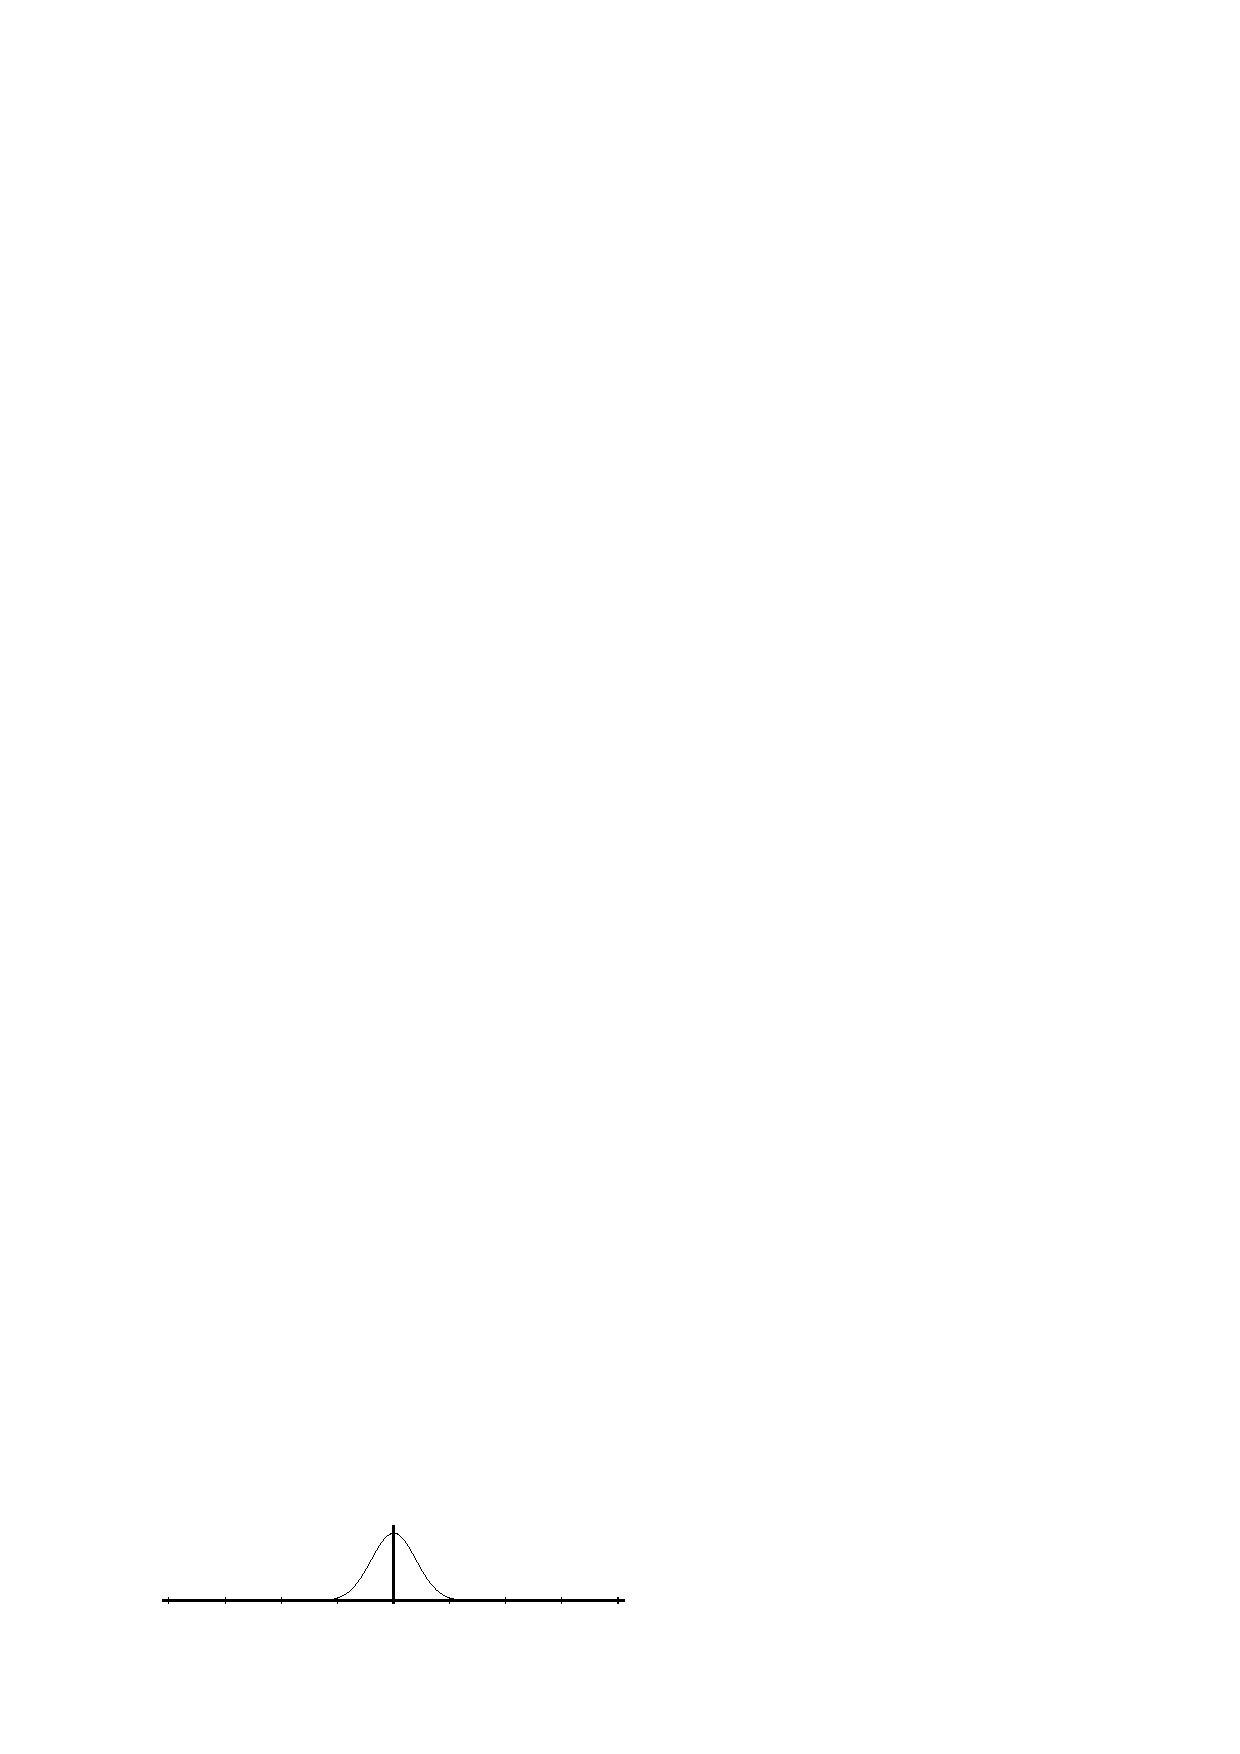
\includegraphics[width=3.8in]{ch2-fg1}
\caption{An encapsulated postscript file.}
\end{center}
\end{figure}


%
% --------------------------------------------------------------
% The second figure was produced by Maple and generated in
% landscape mode.  We need to rotate the figure 90 degrees using
% the angle option.  Note that in this case the height is really
% the width and vice versa.
% --------------------------------------------------------------
%


\begin{figure}[h]   % again, the "h" says to put it here
\begin{center}
%\epsfig{file=ch2-fg2.ps, height=4.5in,width=2in,angle=-90}
\includegraphics[width=3.8in,angle=270]{ch2-fg2.ps}
%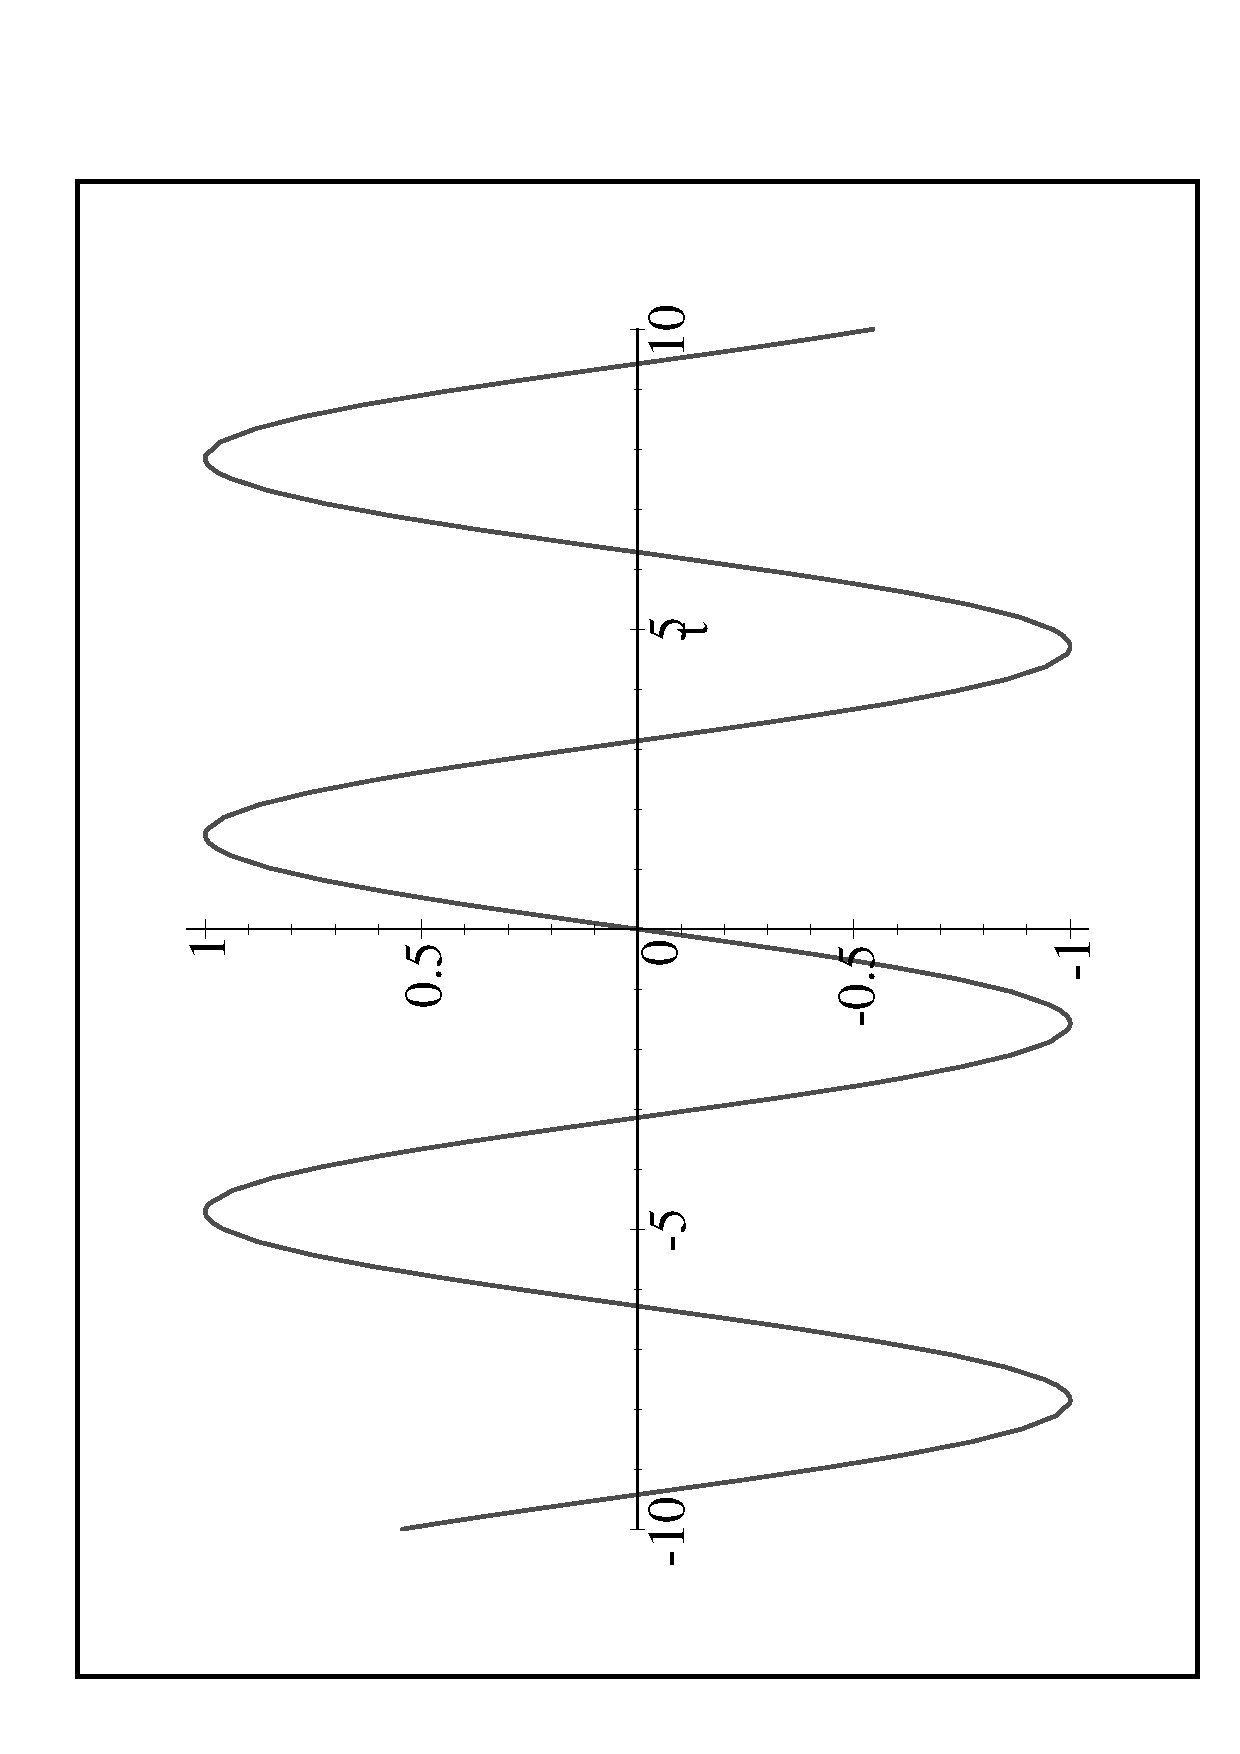
\includegraphics[width=3.8in,angle=270]{ch2-fg2.pdf}
\caption{A second encapsulated postscript file.}
\end{center}
\end{figure}

